\section{Trafiktællinger}
\label{sub:trafiktaellinger}
Dette afsnit tager udgangspunkt i kilden:
\\ http://vej08.vd.dk/mastra/mastradok/dok/TrafiktaellingerPlanUdfoerEfterb.pdf

Trafiktællinger udføres til mange formål. Det gælder alt fra at kontrollere den overordnede vejplanlægning til at undersøge klagesager om for høje trafik hastigheder. Trafiktællinger bruges bl.a. til at finde løsninger til opgaver omhandlende trafiksikkerhed, kapacitet og miljøforhold, samt statistikker over trafikudviklingen og hastigheden af vejnettet. Man kan foretager trafiktællinger manuelt eller ved brug af maskiner.
Manuelle tællinger fungerer ved at personer registrere trafikken på det pågældende sted, ofte ved hjælp af tælleblokke, håndtællere eller håndterminaler. Ved maskine tælling fortages registreringerne automatisk ved brug af et tælleapparat, hvor mennesker ikke medvirker.

\subsection{Manuel tælling}
\label{sub:manuel_taelling}
Manuel tælling er som sagt, hvor det er mennesker der tæller trafikken. Manuel tælling er en god metode, når der ønskes at kende trafikkens specifikke trafikstrømme. Et typisk forløb for manuel tælling er opbygget af 6 trin.
%\\\\
1) Som det første skal formålet for tællingen bestemmes, samt hvilken resultat type, som ønskes af opnå.
%\\\\
Vores formål med trafiktællingen er tælle hvor mange fodgængere, cykelister og billister, som befinder sig inde ved Nytorv og Østerågade. Efterfølgende vil restultaterne blive omregnet  til årsdøgnstrafik ÅDT. Desuden vil der blive noteret hvilken retning trafikanten kom fra og hvilken retning trafikanten begiver sig hen mod. Herved indsamles data, som kan benyttes til at lave et flow kort over trafikken.
%\\\\
2) Der skal besluttes placeringen af tælleposterne, hvor der skal tages hensyn til at tælleren ikke genere trafikken. Tællerne skal også have frit udsyn for parkerende biler, buskaser og lignende under hele tælleperioden. Man skal derfor overveje, om forholdene kan ændre sig undervejs. I trafiktællingen er der observeret ude foran The Harp, som er en bar lige foran fodgængeroverfeltet på figur (??), og ligger ud til Østerågade (evt vis på kort?). Her var der et godt overblik over hele området og ingen former for afskærmninger. Herfra blev alle trafikanter og køretøjer noteret.
%\\\\
3) En af de betydlige usikkerheder ved trafiktællinger er valget af tælleperioden. Der kan være meget stor variation fra dag til dag og time til time, hvis der ønskes at finde årsdøgntrafikken. Der er stor forskel på trafikmængden dels i weekenden kontra hverdage og dels i myldretiden om morgen og eftermiddagen kontra midt på dagen og om aftenen og natten. Manuelle tællinger vare typisk 4, 6 eller 12 timer og sjældent et helt døgn. I undersøgelsen er trafiktællingerne lavet en tirsdag d. 24 november kl. 13:00 til 17:00. Det var vurderet til at være de timer på dagen, hvor der færdes flest trafikanter i området. En af ulemperne ved at observere på en tirsdag i området er, at den stor del af de trafikanterne begiver sig rundt i området, for at benytte sig af de mange shoppingfaciliteter og cafeér. Det er især i weekender at folk vil vælge at gøre dette, og derfor ville det være optimalt, at observere en fredag eftermiddag eller en lørdag. Dog er dette bare en af usikkerhederne i vores opregning af årsdøgstrafikken.
%\\\\
4) Når tælleposterne og tidspunkterne er fastlagt, bestemmes antallet af tællere til posterne, vurderet ud fra trafikmængden på det pågældene sted. Ifølge vejdirektoratet er kvaliteten af resultaterne afhængig af antallet af tællere. Er tælleposterne underbemandet, vil resultaterne blive uanvendelige. Hvis man er uvidende om trafikmængden, og dermed antallet af tæller som er nødvendige, kan man foretage en prøvetælling inden. Da Nytorv/Østerågade er et meget befærdet område, er der valgt 6 personer til at tælle. 2 personer observerer køretøjer og cykler ude foran The Herp, 2 personer observerer fodgængere ovenpå McDonalds, og de sidste 2 personer observerer fodgængere ude foran Baresso. (vis dette på kort)

5) Inden tællerne begynder, er det vigtigt at de er sat sig ind i overstående bestemmelser for tælleforløbet, således der ikke opstår tvivler undervejs. Ligeledes udarbejdes et tælleskema inden tællingen påbegyndes. I undersøgelsen er der lavet et tælleskema i Excel, som henholdsvis angiver de forskellige trafikantgrupper og deres retninger. Herefter noteres der for hvert enkelt trafikant, afhængig af trafikantgruppe og retning.
%\\\\
6) Resultatbehandling af tællingen.
\begin{figure}[htbp]
   \centering
   \begin{adjustbox}{max width=\textwidth}
     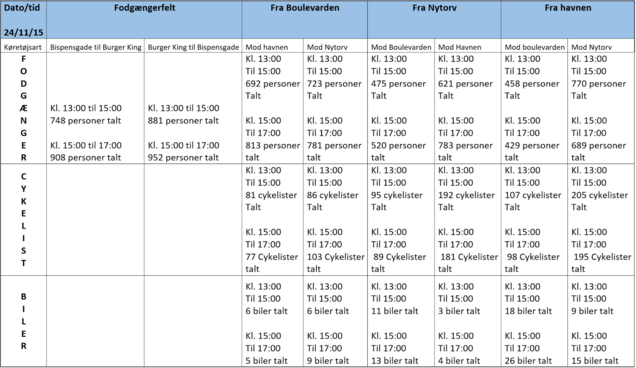
\includegraphics[scale=0.3]{figures/Billederogfigur/resultat.jpg}
  \end{adjustbox}
   \caption{Tabel over trafiktællinger}
   \label{fig:resultat}
 \end{figure}
Der findes ingen omregningsfaktor af fodgængere til ÅDT, derfor er tællingen vurderet, ud fra forholdende på tælledagen. Der blev noteret 2636 fodgængere tirsdag den 24 november kl. 14:00 til 15:00. På dette tidspunkt har skole og gymnasieelever måske fået fri, mens alle som har et 8 til 16 job stadig er på arbejde. Derfor ville der måske have været flere trafikanter, hvis tællingen var lavet senere på den pågældene dag. Til gengæld, hvis tællingerne var taget tidligere og midt i skoletiden, så ville antallet af fodgængere nok være mindre. En anden faktor er, at det regnede mens vi talte. Regnvejret kan have haft en indflydelse på mængden af trafikanter, da det må forventes, at mange vil vælge at benytte sig af området en anden dag. Desuden har dagen og årstiden en stor indflydelse på antallet af fodgængere på Nytorv og Østerågade. Eftersom at der er mange butikker i området, er det ikke bolig– og arbejdetrafik, som benytter sig af området. Det er nærmere folk personlige ærinder eller erhvervstrafikanter. Derfor må det som sagt forventes, at der er flere i weekenderne. I sommerferien vil man også kunne finde meget mere liv, fordi folk mødes, og der bliver afholdt diverse arrangementer nede i byen. Hvis vi skal konkludere på usikkerhederne, er antallet af fodgængere i Østerågade og Nytorv meget situationsafhængig, og resultaterne af trafiktællingerne i rapporten er derfor usikre.
\subsection{Opregning af trafiktællinger til ÅDT}
\label{sub:opregning}
Ved at opregne et antal talte cykler og biler på én dag til ÅDT, vil der altid være en usikkerhed.
I følgende resultatbehandling vil der være fokus på en trafiktælling af cykler og biler ved Nytorv i Aalborg tirsdag d. 24/11 i tidsrummet 13-17. I dette tidsrum er der tale om en blanding af såkaldt bolig/arbejde og by/lokal trafik, da det er i dette tidspunkt, at gennemsnittet af befolkningen får fri fra arbejde og skole, går på indkøb, og i dette tidsrum, at folk skal hjem til sig selv.
Antallet af biler, som vi fik talt i perioden var 104, og antallet af cykler i samme periode var 1408.
For at opregne en trafiktælling, som denne til årsdøgnstrafik, skal man bruge en bestemt formel:
$$ T \times FDT \times FUHDT \times FUDT \times FÅDT = ÅDT $$ eller $$ UDT \times FÅDT = ÅDT$$ , hvor:

$$T = Talt trafik$$

$$UDT = Ugedøgstrafik$$

$$FDT = Opregningsfaktor til døgntrafik i tælleugen$$

$$FUHDT = Opregningsfaktor til ugehverdagsdøgntrafik i tælleugen$$

$$FUDT = Opregningsfaktor til ugedøgntrafik i tælleugen$$

$$FÅDT = Opregningsfaktor til årsdøgntrafik i tælleåret$$

$$FÅR = Opregningsfaktor fra tælleår til andet år$$

Den sidstnævnte formel til at udregne ÅDT’en, er den mest oplagte, da der findes en nem metode at finde frem til UDT, og hernæst skal FÅDT blot aflæses og ganges med UDT, for at vi kan finde ÅDT.

\subsection{ÅDT}
\label{AEDT}
\subsubsection{Cyklernes ÅDT på Nytorv i Aalborg}
\begin{figure}[htbp]
   \centering
   \begin{adjustbox}{max width=\textwidth}
     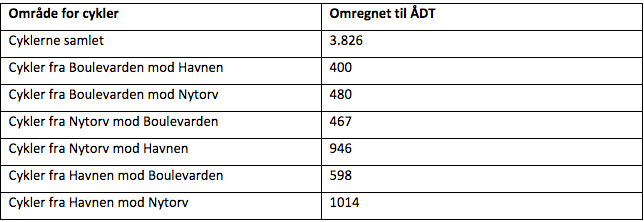
\includegraphics[scale=0.8]{figures/Billederogfigur/cykleradt.jpg}
  \end{adjustbox}
   \caption{Cyklernes ÅDT i Aalborg}
   \label{fig:cykleradt}
 \end{figure}
 
 \subsubsection{Bilernes ÅDT på Nytorv i Aalborg}
 \begin{figure}[htbp]
   \centering
   \begin{adjustbox}{max width=\textwidth}
     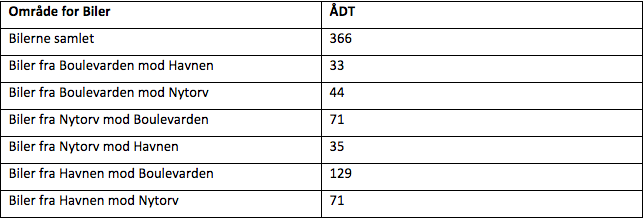
\includegraphics[scale=0.6]{figures/Billederogfigur/bileradt.jpg}
  \end{adjustbox}
   \caption{Bilernes ÅDT i Aalborg}
   \label{fig:bileradt}
 \end{figure}
 
\subsubsection{Flow kort over biler}
\begin{figure}[htbp]
   \centering
   \begin{adjustbox}{max width=\textwidth}
     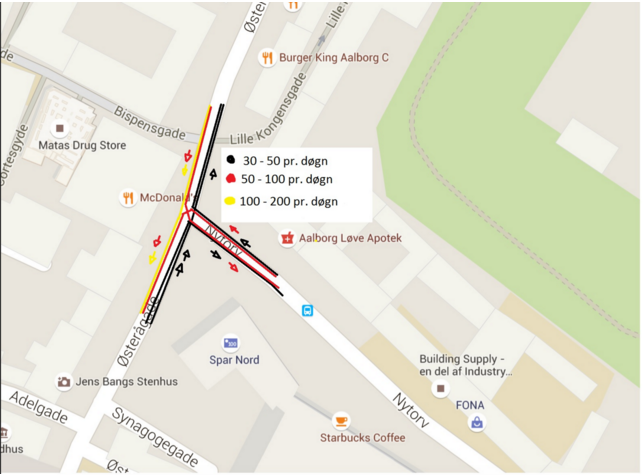
\includegraphics[scale=0.6]{figures/Billederogfigur/bilerflow.jpg}
  \end{adjustbox}
   \caption{Denne illustration viser bilernes flow i løbet af et døgn}
   \label{fig:bilerflow}
 \end{figure}
 
\subsection{Flow kort over cykler}
\begin{figure}[htbp]
   \centering
   \begin{adjustbox}{max width=\textwidth}
     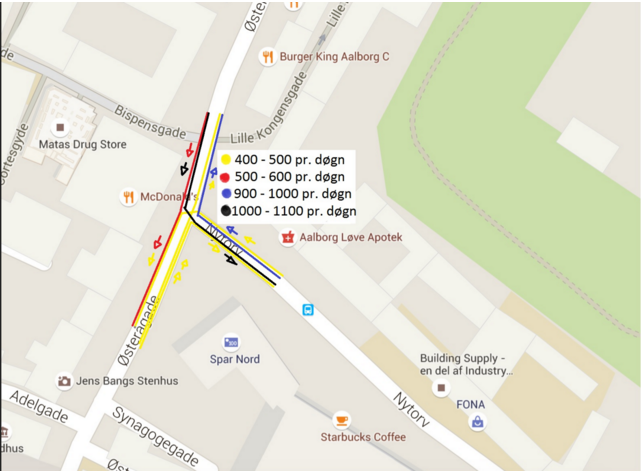
\includegraphics[scale=0.6]{figures/Billederogfigur/cyklerflow.jpg}
  \end{adjustbox}
   \caption{Denne illustration viser cyklernes flow i løbet af et døgn}
   \label{fig:cyklerflow}
 \end{figure}
 
 \subsection{Flow kort over fodgængere}
 \begin{figure}[htbp]
   \centering
   \begin{adjustbox}{max width=\textwidth}
     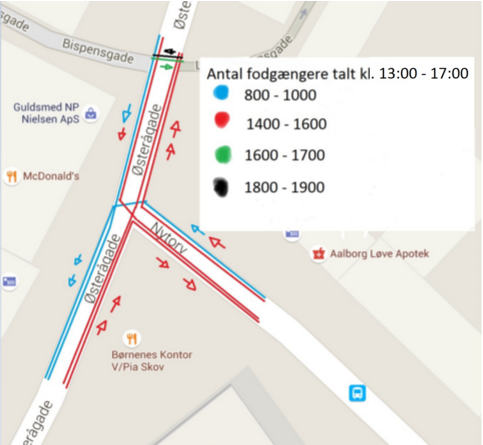
\includegraphics[scale=0.6]{figures/Billederogfigur/fodflow.jpg}
  \end{adjustbox}
   \caption{Denne illustration viser fodgængernes flow i løbet af et døgn}
   \label{fig:fodflow}
 \end{figure}
 
Resultaterne for de opregnede ÅDT-værdier, som er beregnet ud fra bilag ??, kan ses på ~\cref{fig:cykleradt} og ~\cref{fig:bileradt} side \pageref*{fig:cykleradt}, hjælper os til at give et overblik over, hvor mange antal af hver trafikantgruppe, som bevæger sig i de forskellige retninger. På flowkortet er der givet et mere tydeligt billede af disse tal. Som det kan ses på flowkortet over bilerne, ses det ved hjælp af de farvede afmærkninger, at der er flest biler der passerer området kørende fra havnen mod boulevarden. Ligeledes kan vi se på flowkortet over cyklerne, at ruten, som er mest befærdet er fra havnen op mod nytorv. På det sidste flowkort, kan man se, at der er størst trafik i begge retninger over fodgængeroverfeltet. Hvis man sammenligner de tre flowkort, kan man se, at omkring fodgængeroverfeltet på østerågade, er der flest af alle trafikantgrupper lige netop her. Dette resulterer i, at dette også er stedet, hvor der er størst sandsynlighed for, at en eventuel kollision kan finde sted, da der er flest implicerede parter til stede på samme sted, på samme tid, hver dag.